\documentclass[11pt]{article}
\RequirePackage{amsthm,amsmath,amsfonts,amssymb,graphicx,url,placeins,multirow,booktabs,dsfont,bbm,lineno,makecell,enumitem,placeins,url,comment,longtable,footnote,array,mathtools,tabulary,colortbl,siunitx}
\usepackage[utf8]{inputenc}
\usepackage[a4paper, total={6in, 8in}]{geometry}
\usepackage{graphicx}
\usepackage{caption}
\usepackage{float}
\usepackage{setspace}
\usepackage[sorting=none]{biblatex}
\usepackage{hyperref}
\usepackage{subfigure}
\usepackage{pdflscape}
\addbibresource{bibliography.bib} %Import the bibliography file
\setlength{\parindent}{4em}
\renewcommand{\baselinestretch}{2.0}

\title{}
\author{Sourav Bhattacharjee, Ivan Kirev, Samuel Cooper , Frederick Sligo-Young, Kilesh Nundlall}
\date{16/06/2021}

\begin{document}
\begin{titlepage}
    \begin{center}
        \vspace*{6cm}
        \Huge
        {Under the radar: A county level exploration of COVID-19-associated Orphanhood during 2020 in the United States.}
    \end{center}
    \vspace{3cm}
    \large
    \begin{center}
        Sourav Bhattacharjee, Ivan Kirev, Samuel Cooper, Frederick Sligo-Young, Kilesh Nundlall
    \end{center}
\end{titlepage}
\doublespacing

\newpage



\tableofcontents

\newpage
\section{Introduction}

\subsection{Background}\label{s:background}

During the preliminary stages of the ongoing COVID-19 pandemic the primary goals of governments around the world has been to mitigate infections, minimize deaths and support vaccine development and mass vaccination programs.\cite{government_response} However, deaths continue to have impacts years after the event, for example, the effect on a child of losing a primary caregiver may be significant throughout the rest of their life, so the issue of an increasing number of COVID-19 orphans is critically important. 

Deaths from COVID-19 can often occur a short number of weeks after infection so it is difficult for a family to plan for children left behind \cite{global_study}. Whilst it may be possible for some children to be looked after by friends or relatives, others may inevitably be placed in institutional care which results in the most acute difficulties. Studies of orphans placed into institutional care show that the lack of a relationship with a primary caregiver often results behavioral impairment, attachment disorders and lowered IQ\cite{browne}. These effects are similar to those in children that have experienced violence\cite{johnson}. 

The pandemic has affected different groups and boroughs, even within the same city, very differently due to factors such as health, living conditions and job security\cite{triangle} which illustrates the importance to identify exactly which areas have been most affected so help can be more effectively directed their way. Notably, with regards to orphans, the communities which have been particularly struck by the pandemic (poorer, often ethnic minorities) are also the ones where children are more likely to live in multi-generation households and be cared for by vulnerable grandparents. In the whole of the USA, 5.9 percent of households are multi-generational but this varies between states, in Hawaii they make up 11.1 percent, the variance is even larger at county level (see map) hence the loss of a care-giving grandparent due to COVID-19 may also significantly affect the welfare of the child. The frequency of multi-generational living also varies with race, 3.7 \% for non-Hispanic White household compared with 10 \% for Hispanic and American Indian households\cite{housing}.

\begin{figure}[H]
\vspace{20pt}
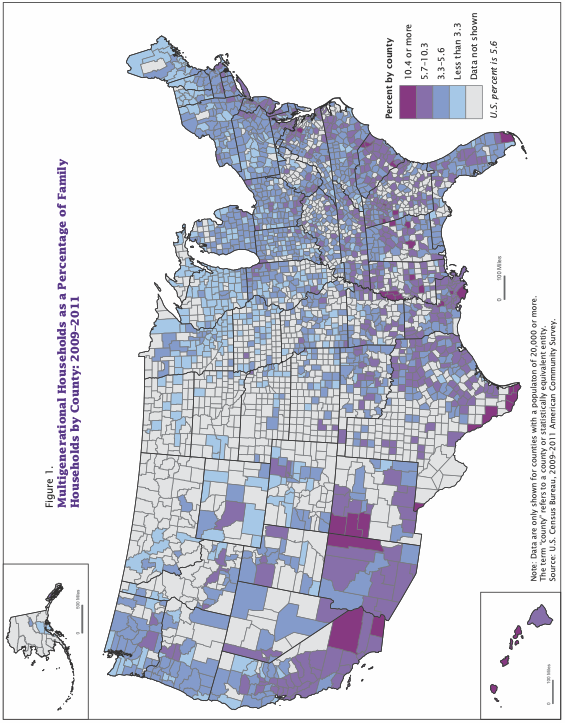
\includegraphics[width=0.45\textwidth, angle = 270]{ImageResults/Households.png}
\centering
\captionof{figure}{Multigenerational Households by County \cite{grandparents}}
\end{figure}

 
Some prior research in the field, including the paper Under the Radar: Global Minimum Estimates for COVID-19-Associated Orphanhood and Deaths Among Caregivers During 2020\cite{global_study} has found estimates for COVID-19 oprhanhood worldwide and explored how the number of orphans are influenced by fertility rates, average age of caregivers, occupation(s) of primary caregiver and presence of grandparents (now 20\% of the world population\cite{grandparents}), however these estimates are unable to determine the number of orphans on a more accurate sub-country level.

\subsection{Preliminary definitions}

To specifically define the goal of our project we first properly define terms "Child", "Orphan" and "Primary caregiver", which are used frequently in the remainder of the report. These definitions are similar to those used in prior research.\cite{global_study}

\noindent
\textbf{Child}: We consider a person to be a child if their age $a$ is in the set $\{0, 1, 2, ..., 17\}$.

\noindent
\textbf{Primary caregiver}: We consider a person to be a primary caregiver for a child if they are one of the following: \label{s:primary caregiver}

\begin{itemize}
    \item The co-residing mother of the child.
    \item The co-residing father of the child.
    \item A co-residing skip-generation grandparent of the child (meaning that the grandparent is directly responsible for the care of the child in the absence of co-residing parents).
    \item A co-residing care-giving grandparent of the child (meaning that the grandparent is directly responsible for the care of the child in the presence of co-residing parents).
\end{itemize}
    
\noindent
\textbf{Orphan}: We consider a person to be an orphan if they are a child and at least one of their primary caregivers have died. \\ 

\noindent
\underline{Note}: In the context of this report we occasionally use the term "COVID-19 Orphan" to refer to orphans for whom at least one primary caregiver has died due to the COVID-19 pandemic.

\subsection{Project goal}
Our goal in this project was to further the development of a statistical model which estimates the number of COVID-19 associated orphans at US county-level, in order to help identify counties associated with a high density of COVID-19 orphans. The county-level accuracy is an improvement over the more general country level estimates found in prior research as described in section \ref{s:background}\cite{global_study}

In this report we detail several aspects of the project, including: (1) the challenges in the sourcing and organization of population and natality data on a county level basis; (2) assumptions and techniques used in the computation of orphans estimate; (3) a visual heat map representation of high and low COVID-19 orphanhood counts and density; (4) a discussion and evaluation of our findings and extensions for further research. 

\section{Methodology and data manipulation}
In this chapter we provide a detailed description of the required acquisition of data and the methodology used throughout the project to compute, to a county-level accuracy, COVID-19 associated orphan-hood estimates. Much of this methodology was already developed for global COVID-19 orphanhood research and implemented through collection of R scripts developed by researchers at Imperial college London\cite{global_study} which we were given access to. Our challenge was to understand and run this methodology as well as make edits to the code to compute our desired estimates for several US states investigated. Our analysis consists of the following four main stages: 

\begin{itemize}
    \item Collecting and processing COVID-19 death data specified for age group, race, sex and county for states in the US (discussed in chapter \ref{s:processing of covid-19 deaths}).
    \item Manipulating county-level population and natality data to compute estimates for expected number of children (discussed in chapter \ref{s:number of children parents}).
    \item Manipulating co-residing grandparents data to compute estimates for the expected number of children. (discussed in chapter \ref{s:number of children grandparents}).
    \item Computing the expected number of orphans at county-level accuracy (discussed in chapter \ref{s:final computation}).
\end{itemize}



\subsection{Data acquisition}\label{s:data_acquisition}

We briefly discuss the various databases we sourced data from and the data storage. The computation of this estimate involved the processing of various data sets including:
\begin{itemize}
    \item COVID-19 deaths data from the National Centre of Health Statistics (NCHS), which was divided into the following datasets:
    \begin{itemize}
        \item Provisional COVID-19 deaths by Sex and Age~\cite{COVID_19_Deaths_by_sex_and_age}
        \item Provisional COVID-19 deaths by county, race and Hispanic origin~\cite{COVID_19_Deaths_by_county_and_race}
    \end{itemize}
    \item Natality data collected from the CDC divided into:
    \begin{itemize}
        \item Male natality data from the 2016-2019 expanded Natality dataset (CDC)~\cite{Male_fertility_data}
        \item Female natality data from the 2003-2006 Natality (CDC)~\cite{Female_fertility_data_2003}, and the 2007-2019 Natality (CDC) datasets~\cite{Female_fertility_data_2019}.
    \end{itemize}
    \item Population data from the CDC, divided into:
    \begin{itemize}
        \item Male population data from the Single race population estimates 2010-2019 database (CDC) for years 2016-2019~\cite{Male_population_data}.
        \item Female population data from the Bridged race population estimates 1990-2019 (CDC) database for years 2003-2019~\cite{Female_population_data}.
    \end{itemize}
    \item Child mortality data for the US from the UNICEF Mortality among children, adolescents and youth aged 5-24 database~\cite{Child_Mortality_Data}.
    \item Co-residing grandparents data from the Grandparents database from the United States Census Bureau~\cite{grandparents_data}.
\end{itemize}
All the data above was collected, appropriately named by the necessary convention and stored in a common git repository. In total we collected over 900 data files consisting of natality and population data from the CDC with a total file size of approximately 700MB.


\subsection{Processing of COVID-19 deaths data}\label{s:processing of covid-19 deaths}
The goal of the first step is to extract the expected number of COVID-19-related deaths by age $a$ (years), sex $s$, race $r$ and county $c$. We denote this quantity by $X_{c,a,r,s}$ and will make use of it in the final computation, described in Section~\ref{s:final computation}. We find this estimate for every combination of 
\begin{subequations}\label{e:deaths_strata}
\begin{align}
    & a \in \{1, 2, ..., 100\} \\ \label{s:1a}
    & s \in \{\textrm{Male}, \textrm{Female}\}\\ \label{s:1b}
    & r \in \{\textrm{Hispanic, Non-Hispanic White, Non-Hispanic Black, Non-Hispanic Asian},\\  \label{s:1c}
    & \quad\quad\quad \textrm{Non-Hispanic American Indian or Alaska Native}\}
\end{align}
\end{subequations}
for counties $c$ within chosen US states.

We find $X_{c,a,r,s}$ almost directly from the CDC website, however, since the data file containing all of the combinations in~\eqref{e:deaths_strata} is too large and therefore the website does not allow us to download it all at once, we split the data into two parts, the first consisting of the sex and age\cite{COVID_19_Deaths_by_sex_and_age} categories and the second of county and race.\cite{COVID_19_Deaths_by_county_and_race}

Now given these two data sets, our next step is to combine them. To be able to do this, we assume that COVID-19 deaths by (Sex and Age group) and (County and Ethnicity) are independent. Hence to get the expected number of people dying from COVID-19 for  a given sex, age, ethnicity and from a certain county, we simply multiply the probability a person of a person of a chosen (Sex and Age group) has died from COVID-19 with the number of people in a chosen (County and Ethnicity) for the same state in the US. Doing this for each of the possible combination, we obtain our final COVID-19 deaths by Sex, Age Group, County and Ethnicity.

Due to missing data for COVID-19 death counts which are below $10$, a small modification was needed to be done to the data. This consists of replacing these empty values with random integers sampled from $1-9$. This assumption does not affect the final results significantly since it only amends small integers and also allows us to proceed with the new data. 


\subsection{Expected number of children based on natality and population data}\label{s:number of children parents}

The second stage of the computation process involved finding estimates for the expected number of children aged between 0-17 years that a person of age $a$, race $r$, sex $s$ and from county $c$ has in 2020. We denote this quantity by $Y_{c,a,r,s}$ for ages $a$, sexes $s$ and races $r$ described in the same combinations as in~\eqref{e:deaths_strata} in chapter \ref{s:processing of covid-19 deaths} for counties $c$ in chosen US states. 

To estimate $Y_{c,a,r,s}$, we first computed fertility estimates $f_{c,a,r,s, y}$ separately across different age groups $a$, sexes $s$, races $r$ and counties $c$ for years $y$ from 2003-2019. We calculated $f_{c,a,r,s, y}$ using
\begin{equation}
    f_{c, a, r, s, y}= \frac{b_{c,a,r,s, y}}{p_{c,a,r,s, y}}
\end{equation}
where $b_{c, a, r, s, y}$ is the total number of births in county $c$ with parent age in age group $a$, parent sex $s$, and parent race $r$, for year $y$ and $p_{c,a,r,s, y}$ is the total number of people in county $c$ in age group $a$, of sex $s$, and of race $r$, for year $y$.

We only calculated fertility values for women between the ages of 15-50 years and for men between the ages of 15-60 years assuming that men and women outside these age categories are infertile, hence $f_{c, a, r, s, y} = 0$ if $a \notin\{15, ..., 50\} $ and $s = \textrm{female}$ or if $a \notin\{15, ..., 60\}$ and $s = \textrm{male}$. To obtain our desired count for $Y_{c,a,r,s}$ we just compute:
\begin{equation}
    Y_{c,a,r,s} = \sum_{y \in \{2003, ..., 2019\}} f_{c, a, r, s, y}.
\end{equation}

The data required for this computation was acquired from various freely available natality and population databases published by the (CDC) mentioned in \ref{s:data_acquisition}, however there were important differences in the available data sets for males and females as well as across different states in the US.

The female natality data was available for all years from 2003-2019 for various states in the US and was collected separately from the Natality 2003-2006 and Natality 2007-2019 databases (see \ref{s:data_acquisition}). However, for both these databases births data was only available for counties of population $\geq 100,000$. Furthermore, counties with fewer than 10 births for any combination of sex, race and age group had suppressed counts. If the corresponding population data for this county we available we instead used the mean fertility for women across all other counties within the same state for which natality data was available as a replacement estimate.

We conducted similar data acquisition and processing steps for males. However natality data was only available from 2016-2019, which we sourced from the  2016-2019 expanded Natality database. To overcome this we processed male fertility calculations only for 2016-2019 (in the same method as female fertility calculations but using population data for males from the CDC Single-Race Population Estimates 2010-2019 database) and used a Poisson general linear model to extrapolate fertility for men for the missing years 2003-2015 using female fertility data instead. To compute the fertility for men between the ages of 50-60 (since female fertility is 0 for these ages), we instead assumed the same fertility as men aged 45-49.

We further corrected our computed expected number of children estimates by taking child mortality into account which we computed from US child mortality data for age groups 0-4, 5-9, 10-14 and 15-19 which we collected from UNICEF child mortality data for the US.

\subsection{Expected number of children for which a co-residing grandparent is a primary caregiver}\label{s:number of children grandparents}

In Section~\ref{s:number of children parents} we calculated the expected number of children (aged between 0 - 17) one person is expected to have in 2020 across age, race, sex and county. This provides information about fathers and mothers which, as mentioned in \ref{s:primary caregiver}, make up two of the components of "primary caregivers". 

Within this section we consider the other two components of primary caregivers and detail our method for computing estimates for the expected number of children a co-residing grandparent of age $a$, race $r$, sex $s$ and living in county $c$ is a primary caregiver of. We denoted this as $Z_{c, a, r, s}$ with race and sex categories the same defined in section \ref{s:processing of covid-19 deaths}, however the ages are slightly different since  grandparents tend to be between 30-100 years. Outside this age range, we set $Z_{c, a, r, s} = 0$.

To estimate $Z_{c, a, r, s}$, we used co-residing grandparents data sourced from the United States Census Bureau\cite{grandparents_data} and counted the proportion of grandparents that are either: skip-generation grandparents or co-residing care-giving grandparents by grandparent race, county of residence and sex of grandparent. We then multiplied this proportion by the population for different grandparent ages to find the number of primary caregiver grandparents. 

Due to the unavailability of data stating the exact number of children a co-residing grandparent is a caregiver for, we assumed that each co-residing grandparent is responsible for exactly one child aged 0-17 years old and so used our estimate of the number of primary caregiver grandparents as an estimate of $Z_{c, a, r, s}$ for the appropriately specified country of residence $c$, age of grandparent $a$, race of grandparent $r$ and sex of grandparent $s$. The method of computation of $Z_{c, a, r, s}$ naturally causes it to be an underestimate since grandparents may be caregivers for more than one child.

Using similar methods to Section \ref{s:number of children parents}, we also correct the expectation for child mortality using the same UNICEF child mortality data\cite{Child_Mortality_Data} to derive our final estimate for the expected number of children a co-residing grandparent of a certain age is a caregiver for.

\subsection{Final computation of the expected number of orphans to a county-level accuracy}\label{s:final computation}
The final step computes the expected number of orphaned children due to loss of caregivers, based on the results obtained in the previous steps. Essentially, the way we do this is, for a given person with characteristics age $a$, sex $s$, race, $r$ and from county $c$, we multiply the expected number of COVID-19 deaths  $X_{c,a,r,s}$ by the expected number of children a person with the same categories is expected to have, $Y_{c,a,r,s}$. Similarly, we multiply $X_{c,a,r,s}$ by the expected number of children for which a co-residing grandparent is a primary caregiver, $Z_{c,a,r,s}$, and we add the two results together to obtain the total expected number of orphans, $T_{c,a,r,s}$,
\begin{equation}
T_{c,a,r,s} = X_{c,a,r,s} Y_{c,a,r,s} + X_{c,a,r,s} Z_{c,a,r,s}.
\end{equation}
To avoid over-counting, we adjust the total number of orphans who have lost a father or a mother by subtracting the expected number of orphans who have lost both parents. We then do similar adjustment for the co-residing grandparents and denote the new total by $T^{adj}$.

Finally, to count the total number of orphans in a given county, we simply sum the adjusted total expectation over the two groups by age, and sex,
\begin{equation}
    T_{c,r} = \sum_a  \sum_s T^{adj}_{c,a,r,s},
\end{equation}
where $a \in \{15 - 24, \dots, 75-84, 85+\}$ and $s \in \{\textrm{Male}, \textrm{Female}\}$.
We get a specific result for each county and race, however in the final part of the code we sum over all races to obtain the total number of orphans for each county,
\begin{equation}\label{e:orphans_by_county}
    T_c = \sum_r T_{c,r},
\end{equation}
where we sum over the racial groups Hispanic, Non-Hispanic White, Non-Hispanic Black, Non-Hispanic Asian, and Non-Hispanic American Indian or Alaska Native. Equation~\eqref{e:orphans_by_county} is used in the total number of orphan maps in Section \ref{s:results} and to derive the density for a county $s$ $d_{c}$, we simply divide this count by the population of minors in the county:
\begin{equation}
    d_{c} = \frac{T_{c}}{\sum_{a\in\{0, 1, ..., 17\}}\sum_{r, s} p_{c, a, r, s}}
\end{equation}

Using these computations we are able to generate visual heat map representations as shown in \ref{s:results}.


%\newgeometry{top=3cm, bottom = 4cm}
%\restoregeometry

\section{Results}\label{s:results}
\subsection{County Results}
We managed to knit out computations into an interactive HMTL file where one can view heat maps for each state we have successfully run the code for. We display both the total number of orphans or the number orphans per 100,000 minors in the county based for these states. By hovering over the counties in a state one can view the estimated number of orphans in that specific county, so you can get back the specific number, rather than just the range indicated on the figure legends. Counties for which computations were unsuccessful due to missing data are left as NA and are coloured grey.
%own page: consider joining with the previous: latex to fiddly to put easily on the pages with the graphs...

\def\fillandplacepagenumber{%
 \par\pagestyle{empty}%
 \vbox to 0pt{\vss}\vfill
 \vbox to 0pt{\baselineskip0pt
   \hbox to\linewidth{\hss}%
   \baselineskip\footskip
   \hbox to\linewidth{%
     \hfil\thepage\hfil}\vss}}

\begin{landscape}
\thispagestyle{empty}
\begin{figure}[h]
\subsubsection*{Alaska}
\hspace*{-3cm}
\begin{minipage}{.8\textwidth}
    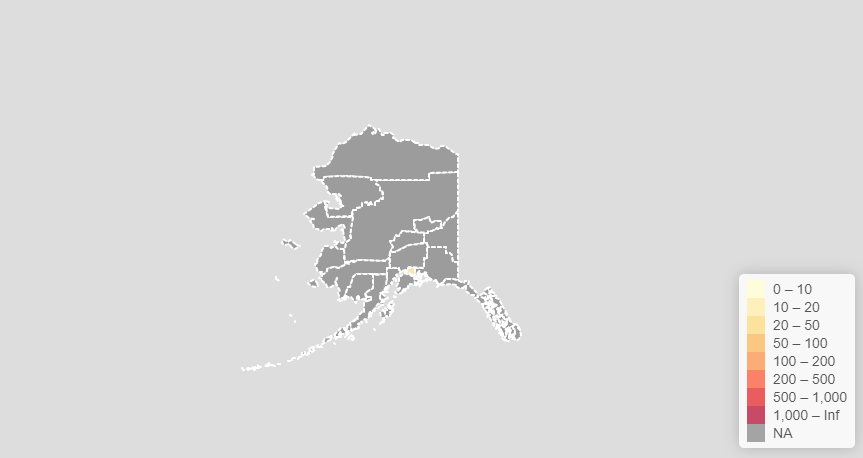
\includegraphics[width=.95\textwidth]{ImageResults/AlaskaTotal.PNG}
    \captionof{figure}{Alaska: Heat-map of Total Number of Orphans}
\end{minipage}%
\begin{minipage}{.8\textwidth}
    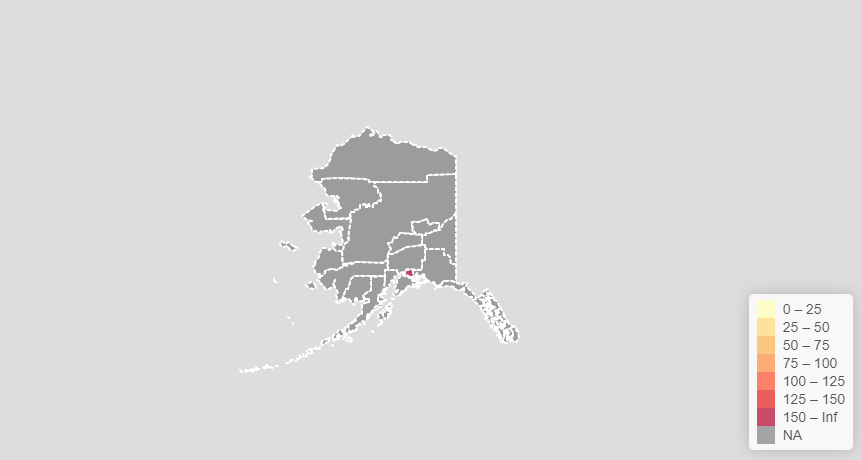
\includegraphics[width=.95\textwidth]{ImageResults/Alaska100k.PNG}
    \captionof{figure}{Alaska: Number of Orphans per 100k Minors}
\end{minipage}
\subsubsection*{Arizona}
\vfill
\hspace*{-3cm}
\begin{minipage}{.8\textwidth}
    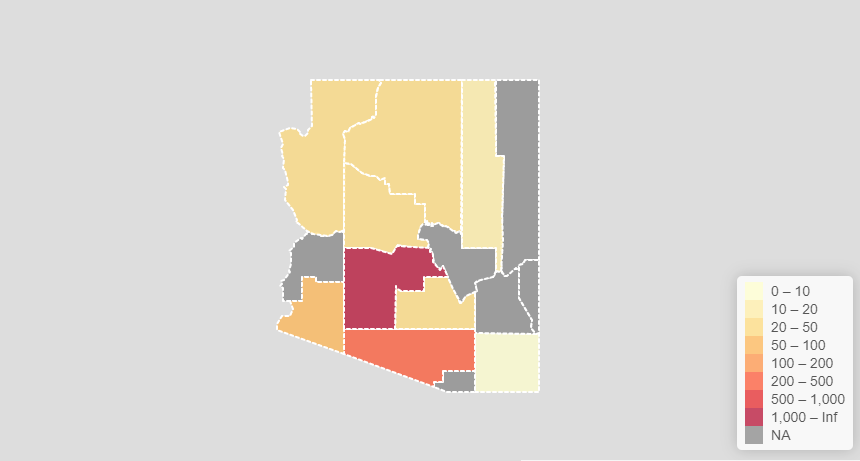
\includegraphics[width=.95\textwidth]{ImageResults/ArizonaTotal.PNG}
    \captionof{figure}{Arizona: Heat-map of Total Number of Orphans}
\end{minipage}%
\begin{minipage}{.8\textwidth}
    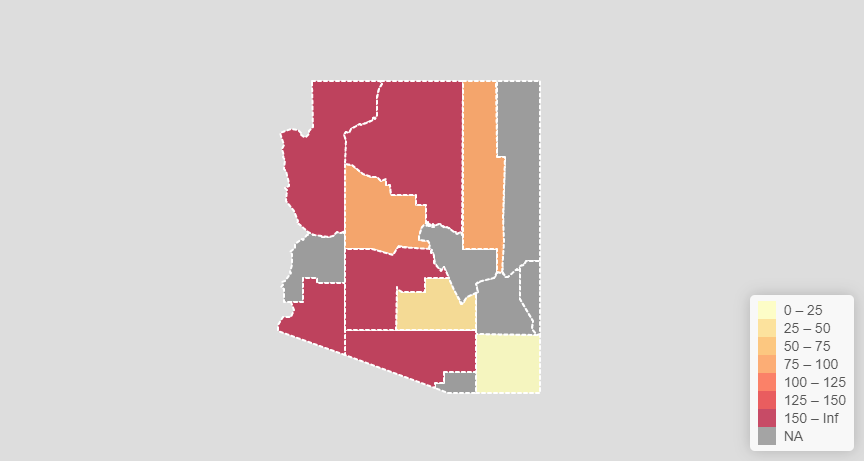
\includegraphics[width=.95\textwidth]{ImageResults/Arizona100k.PNG}
    \captionof{figure}{Arizona: Number of Orphans per 100k Minors}
    \label{fig:Ariz100k}
\end{minipage}
\fillandplacepagenumber
\end{figure}
\end{landscape}

\begin{landscape}
\thispagestyle{empty}
\begin{figure}[h]
\subsubsection*{California}
\hspace*{-3cm}
\begin{minipage}{.8\textwidth}
    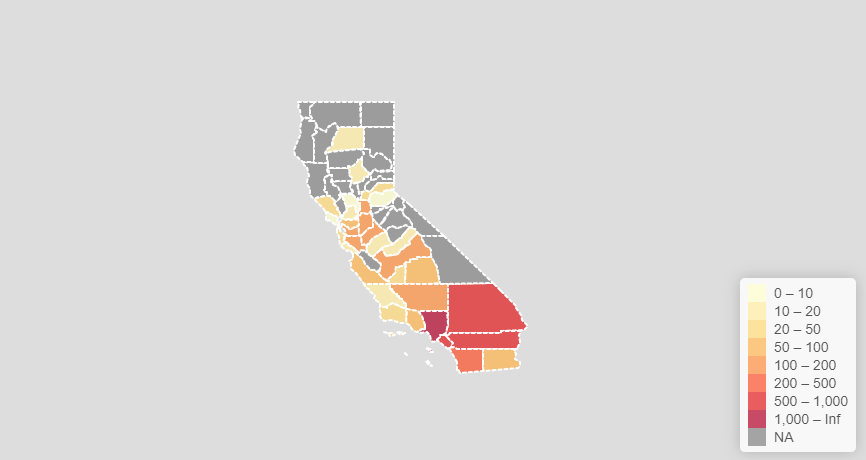
\includegraphics[width=.95\textwidth]{ImageResults/CaliforniaTotal.PNG}
    \captionof{figure}{California: Heat-map of Total Number of Orphans}
\end{minipage}%
\begin{minipage}{.8\textwidth}
    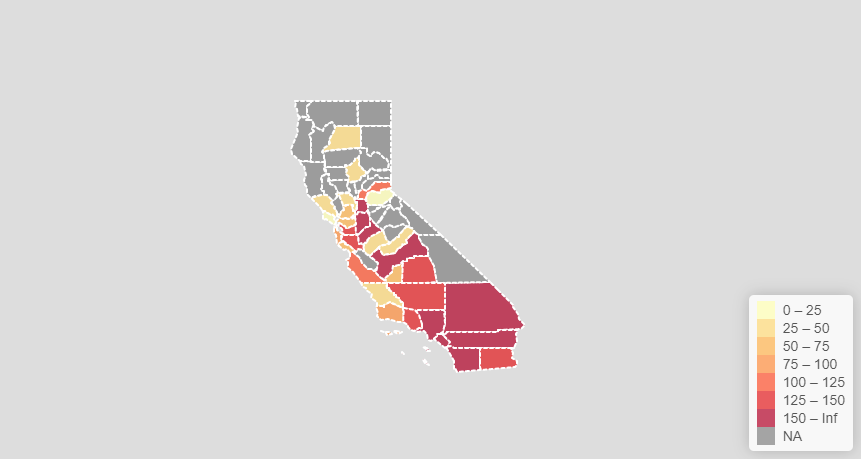
\includegraphics[width=.95\textwidth]{ImageResults/California100k.PNG}
    \captionof{figure}{California: Number of Orphans per 100k Minors}
    \label{fig:Cali100k}
\end{minipage}
\subsubsection*{Connecticut}
\vfill
\hspace*{-3cm}
\begin{minipage}{.8\textwidth}
    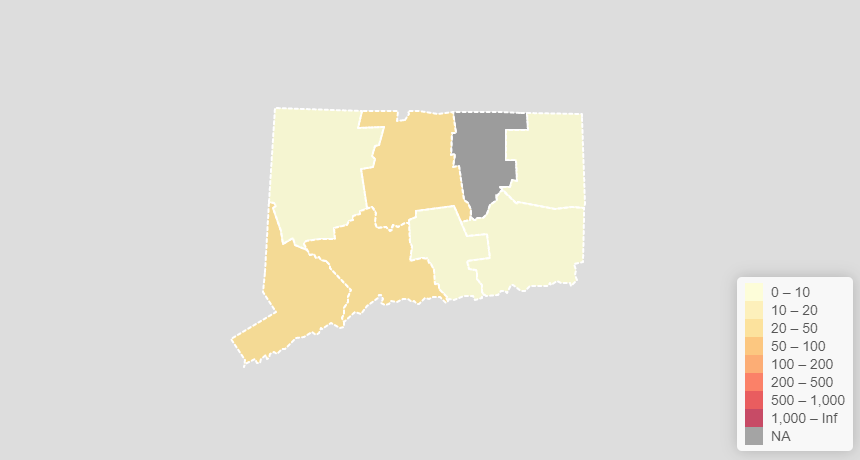
\includegraphics[width=.95\textwidth]{ImageResults/ConnecticutTotal.PNG}
    \captionof{figure}{Connecticut: Heat-map of Total Number of Orphans}
\end{minipage}%
\begin{minipage}{.8\textwidth}
    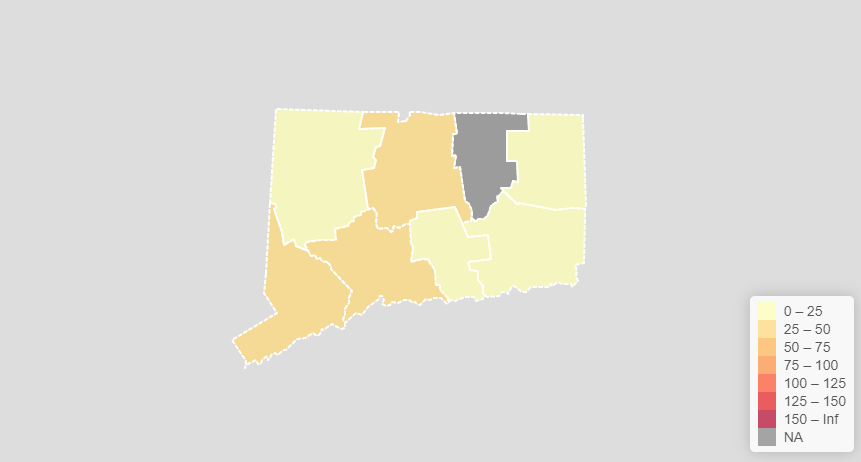
\includegraphics[width=.95\textwidth]{ImageResults/Connecticut100k.PNG}
    \captionof{figure}{Connecticut: Number of Orphans per 100k Minors}
\end{minipage}
\fillandplacepagenumber
\end{figure}
\end{landscape}

\begin{landscape}
\thispagestyle{empty}
\begin{figure}[h]
\subsubsection*{D.C.}
\hspace*{-3cm}
\begin{minipage}{.8\textwidth}
    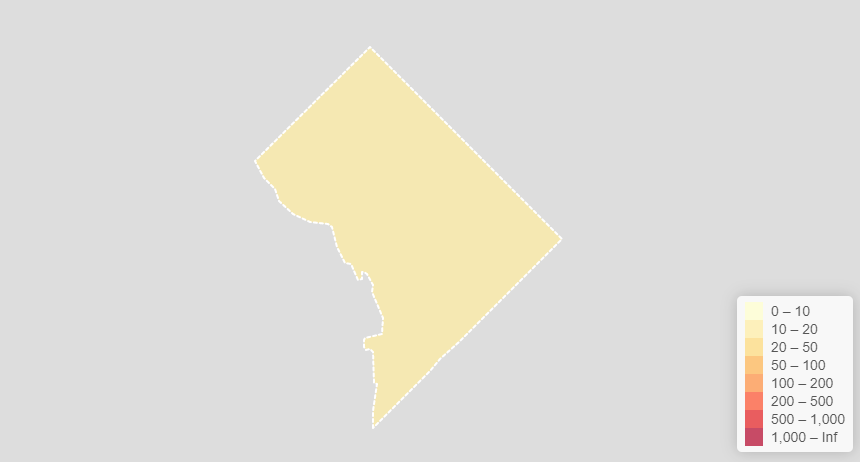
\includegraphics[width=.95\textwidth]{ImageResults/DCTotal.PNG}
    \captionof{figure}{D.C.: Heat-map of Total Number of Orphans}
\end{minipage}%
\begin{minipage}{.8\textwidth}
    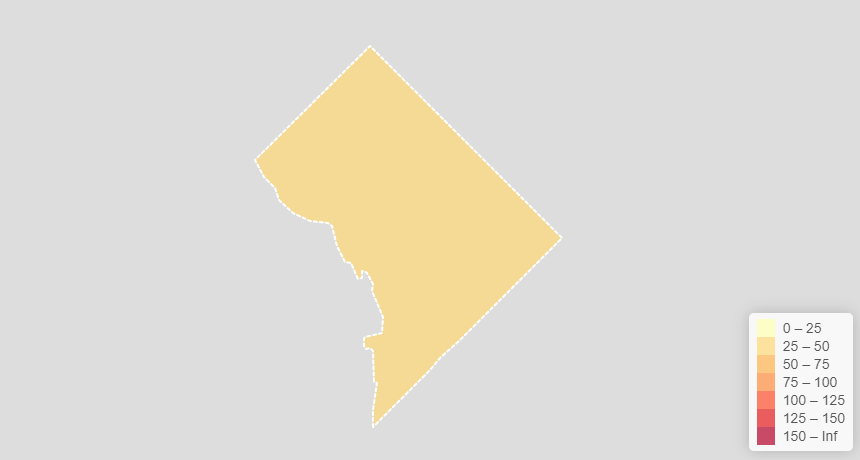
\includegraphics[width=.95\textwidth]{ImageResults/DC100k.PNG}
    \captionof{figure}{D.C.: Number of Orphans per 100k Minors}
\end{minipage}
\subsubsection*{Hawaii}
\vfill
\hspace*{-3cm}
\begin{minipage}{.8\textwidth}
    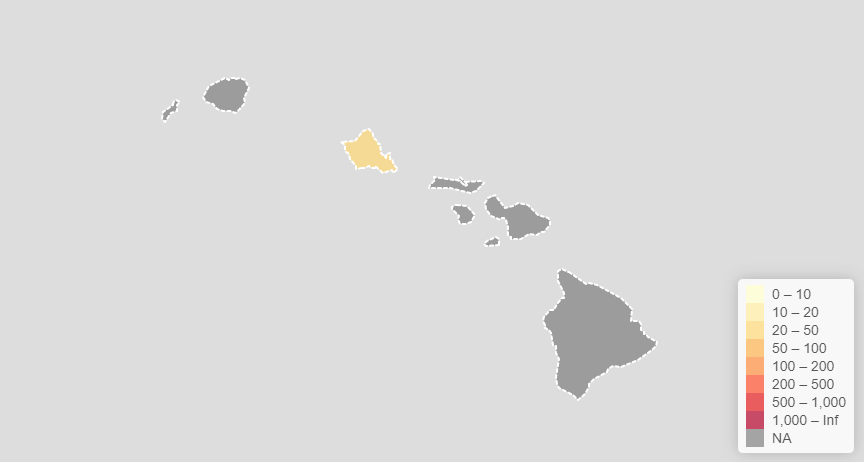
\includegraphics[width=.95\textwidth]{ImageResults/HawaiiTotal.PNG}
    \captionof{figure}{Hawaii: Heat-map of Total Number of Orphans}
\end{minipage}%
\begin{minipage}{.8\textwidth}
    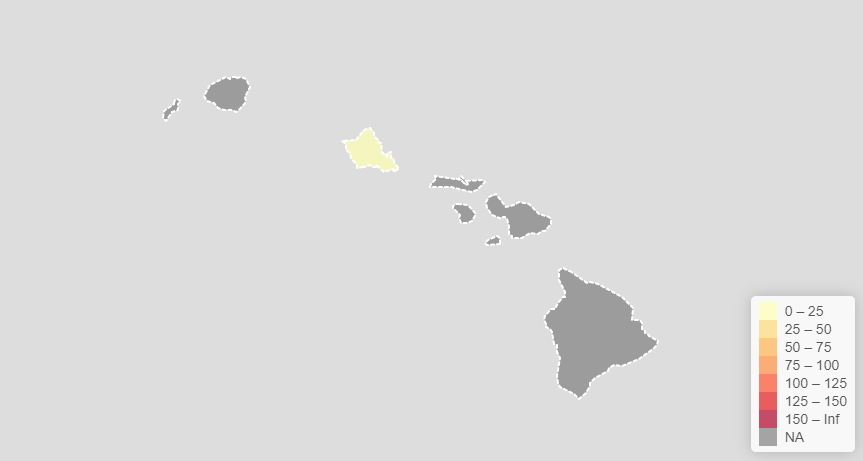
\includegraphics[width=.95\textwidth]{ImageResults/Hawaii100k.PNG}
    \captionof{figure}{Hawaii: Number of Orphans per 100k Minors}
\end{minipage}
\fillandplacepagenumber
\end{figure}
\end{landscape}

\begin{landscape}
\thispagestyle{empty}
\begin{figure}[h]
\subsubsection*{Idaho}
\hspace*{-3cm}
\begin{minipage}{.8\textwidth}
    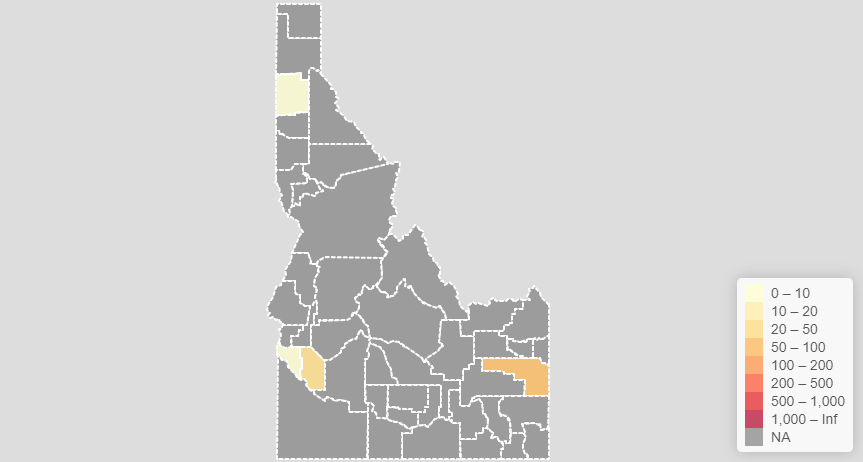
\includegraphics[width=.95\textwidth]{ImageResults/IdahoTotal.PNG}
    \captionof{figure}{Idaho: Heat-map of Total Number of Orphans}
\end{minipage}%
\begin{minipage}{.8\textwidth}
    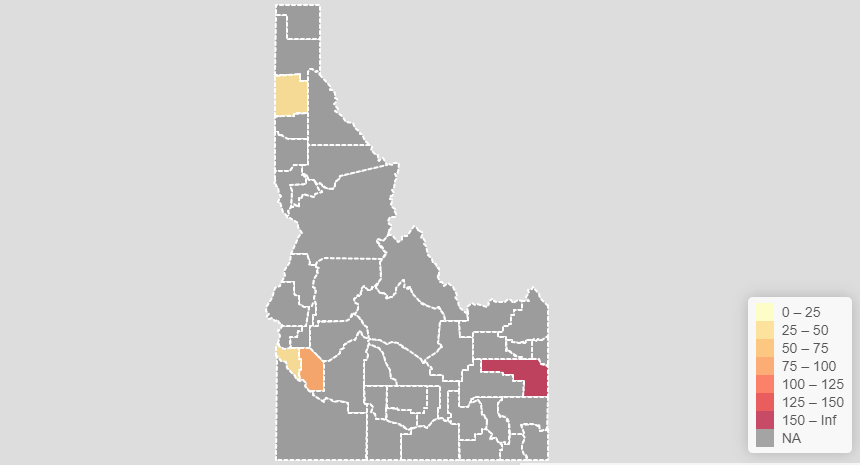
\includegraphics[width=.95\textwidth]{ImageResults/Idaho100k.PNG}
    \captionof{figure}{Idaho: Number of Orphans per 100k Minors}
\end{minipage}
\subsubsection*{Maryland}
\vfill
\hspace*{-3cm}
\begin{minipage}{.8\textwidth}
    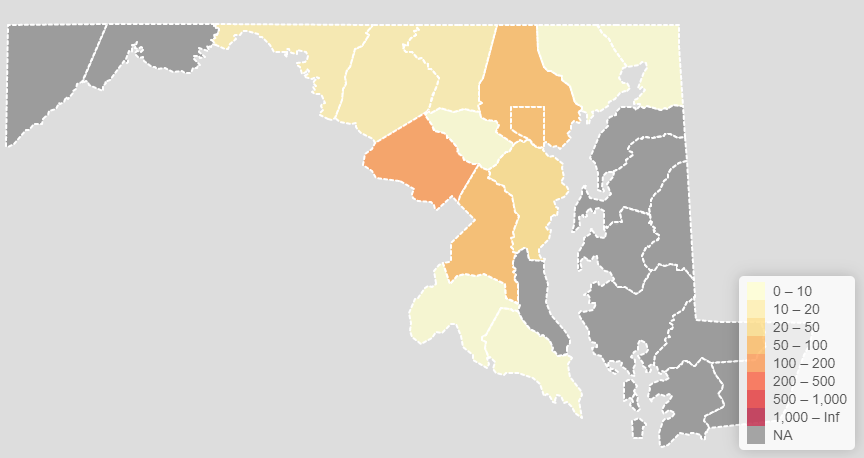
\includegraphics[width=.95\textwidth]{ImageResults/MarylandTotal.PNG}
    \captionof{figure}{Maryland: Heat-map of Total Number of Orphans}
\end{minipage}%
\begin{minipage}{.8\textwidth}
    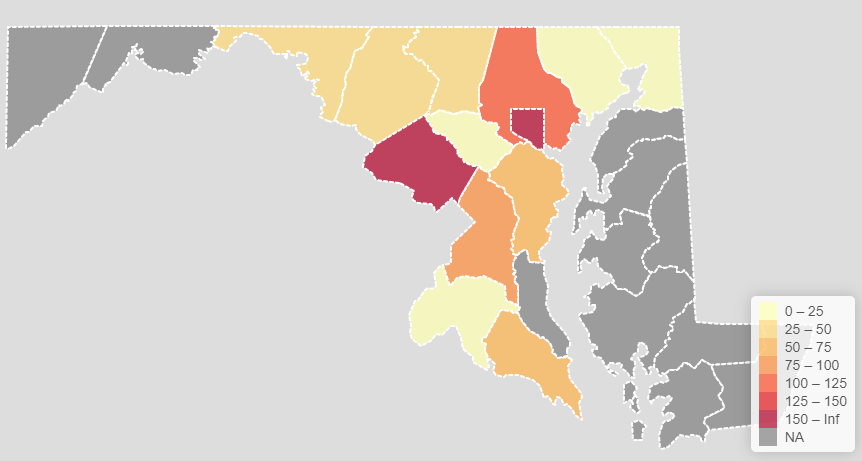
\includegraphics[width=.95\textwidth]{ImageResults/Maryland100k.PNG}
    \captionof{figure}{Maryland: Number of Orphans per 100k Minors}
    \label{fig:Mary100k}
\end{minipage}
\fillandplacepagenumber
\end{figure}
\end{landscape}

\begin{landscape}
\thispagestyle{empty}
\begin{figure}[h]
\subsubsection*{Massachusetts}
\hspace*{-3cm}
\begin{minipage}{.8\textwidth}
    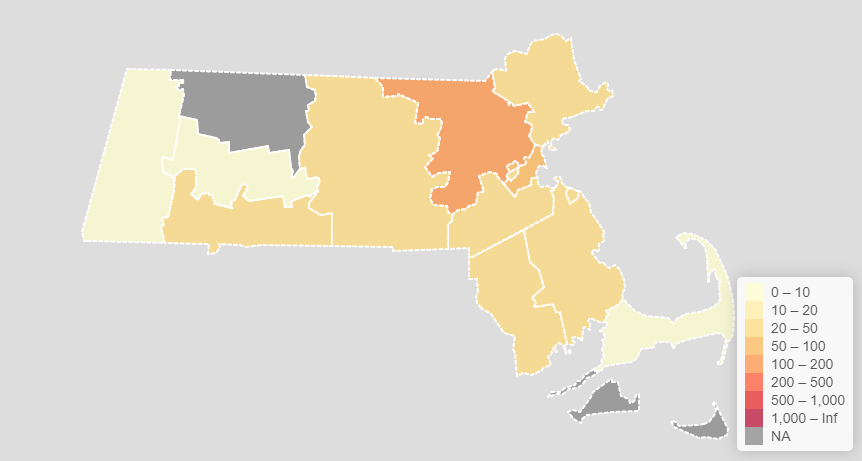
\includegraphics[width=.95\textwidth]{ImageResults/MassachusettsTotal.PNG}
    \captionof{figure}{Massachusetts: Heat-map of Total Number of Orphans}
\end{minipage}%
\begin{minipage}{.8\textwidth}
    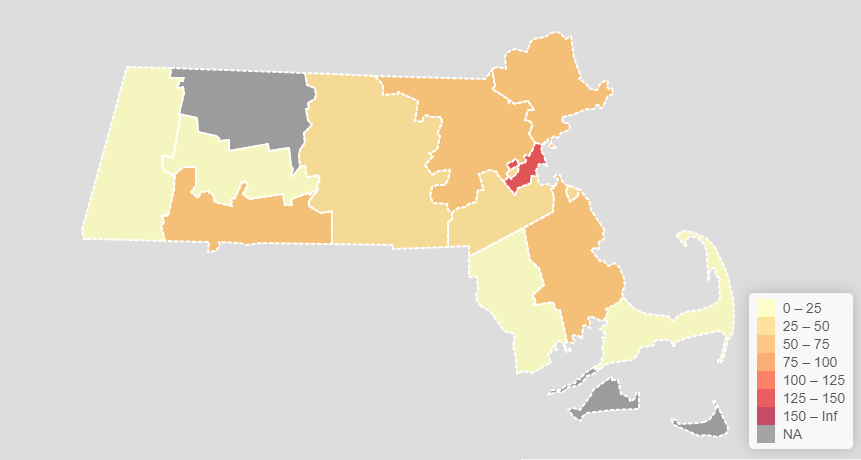
\includegraphics[width=.95\textwidth]{ImageResults/Massachusetts100k.PNG}
    \captionof{figure}{Massachusetts: Number of Orphans per 100k Minors}
    \label{fig:Mass100k}
\end{minipage}
\subsubsection*{Nevada}
\vfill
\hspace*{-3cm}
\begin{minipage}{.8\textwidth}
    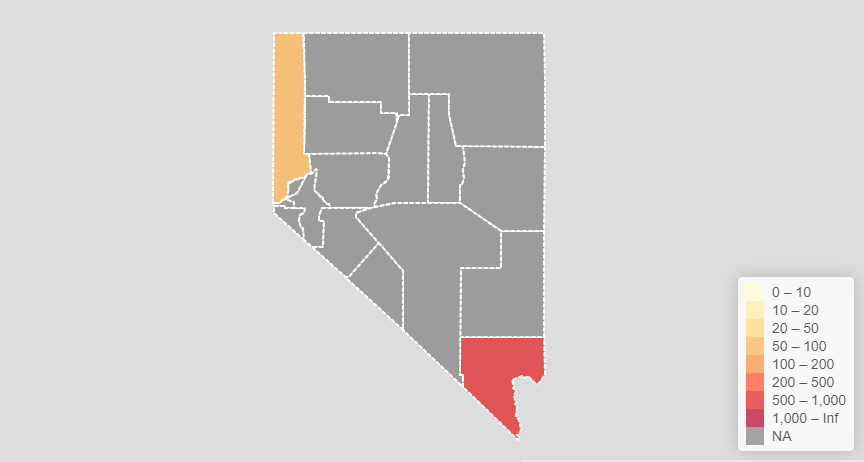
\includegraphics[width=.95\textwidth]{ImageResults/NevadaTotal.PNG}
    \captionof{figure}{Nevada: Heat-map of Total Number of Orphans}
\end{minipage}%
\begin{minipage}{.8\textwidth}
    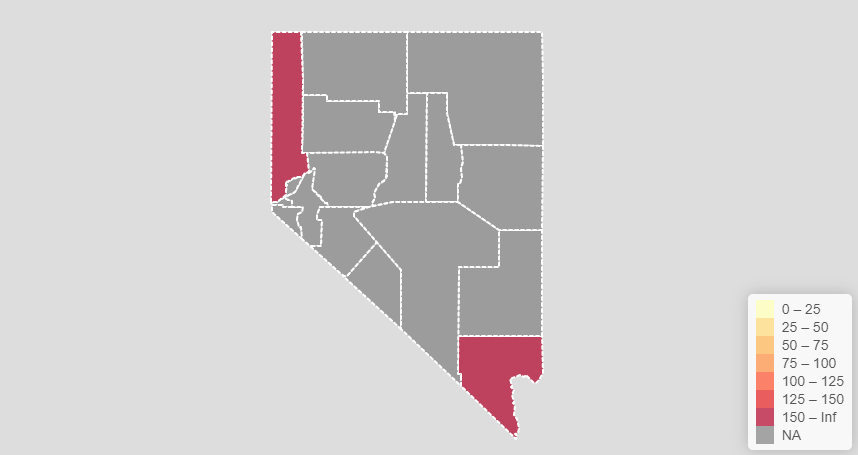
\includegraphics[width=.95\textwidth]{ImageResults/Nevada100k.PNG}
    \captionof{figure}{Nevada: Number of Orphans per 100k Minors}
\end{minipage}
\fillandplacepagenumber
\end{figure}
\end{landscape}

\begin{landscape}
\thispagestyle{empty}
\begin{figure}[h]
\subsubsection*{New Hampshire}
\hspace*{-3cm}
\begin{minipage}{.8\textwidth}
    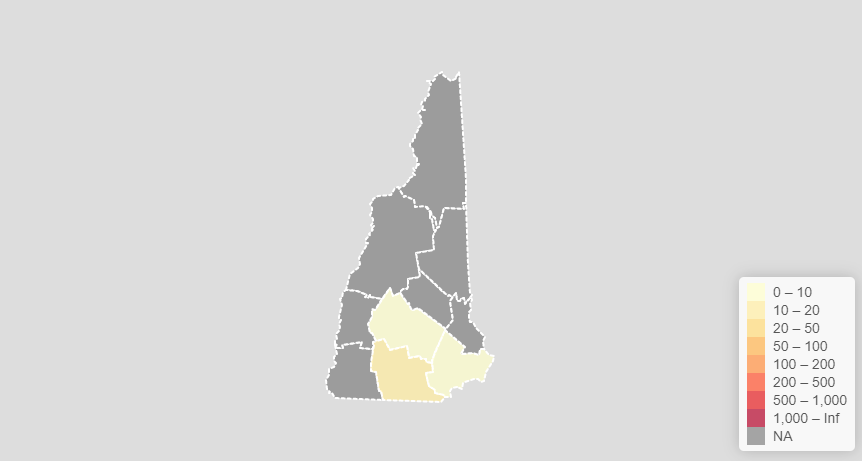
\includegraphics[width=.95\textwidth]{ImageResults/NewHampshireTotal.PNG}
    \captionof{figure}{New Hampshire: Heat-map of Total Number of Orphans}
\end{minipage}%
\begin{minipage}{.8\textwidth}
    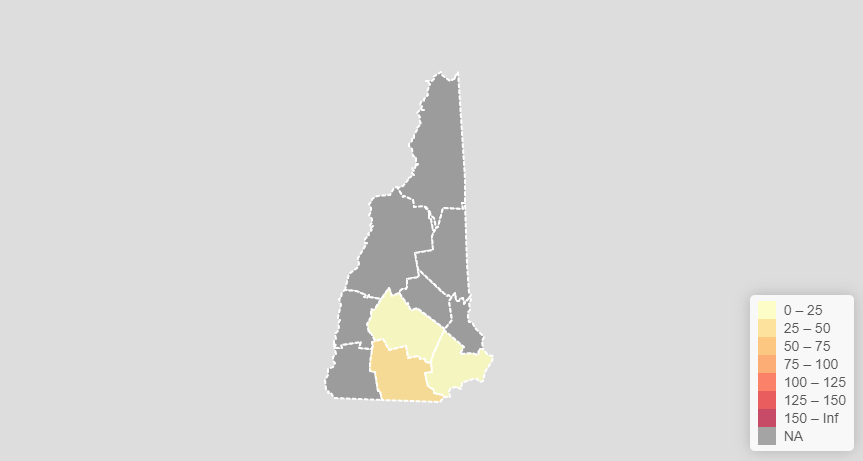
\includegraphics[width=.95\textwidth]{ImageResults/NewHampshire100k.PNG}
    \captionof{figure}{New Hampshire: Number of Orphans per 100k Minors}
\end{minipage}
\subsubsection*{New Jersey}
\vfill
\hspace*{-3cm}
\begin{minipage}{.8\textwidth}
    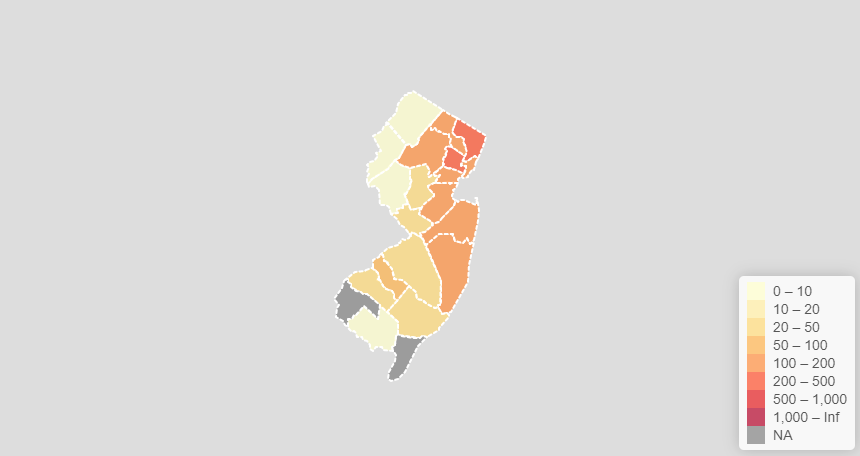
\includegraphics[width=.95\textwidth]{ImageResults/NewJerseyTotal.PNG}
    \captionof{figure}{New Jersey: Heat-map of Total Number of Orphans}
\end{minipage}%
\begin{minipage}{.8\textwidth}
    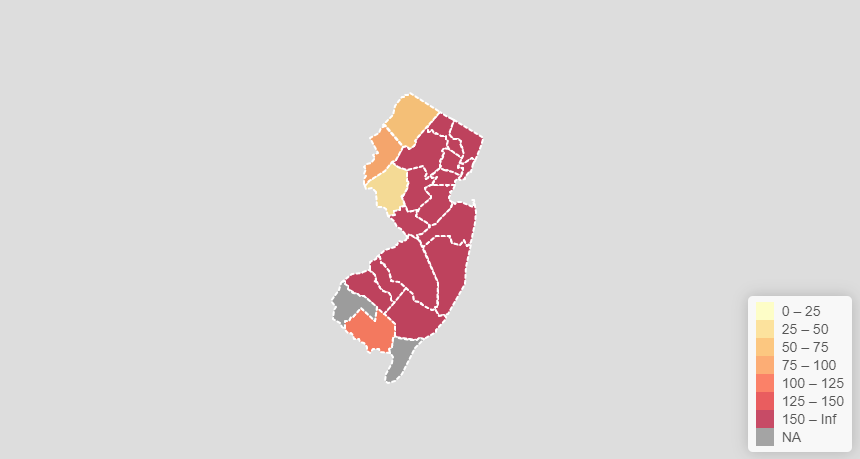
\includegraphics[width=.95\textwidth]{ImageResults/NewJersey100k.PNG}
    \captionof{figure}{New Jersey: Number of Orphans per 100k Minors}
    \label{fig:Newj100k}
\end{minipage}
\fillandplacepagenumber
\end{figure}
\end{landscape}

\begin{landscape}
\thispagestyle{empty}
\begin{figure}[h]
\subsubsection*{Rhode Island}
\hspace*{-3cm}
\begin{minipage}{.8\textwidth}
    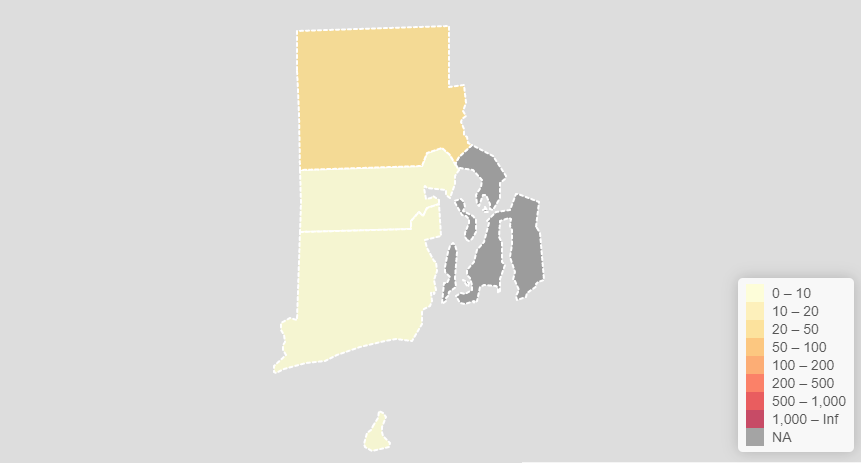
\includegraphics[width=.95\textwidth]{ImageResults/RhodeIslandTotal.PNG}
    \captionof{figure}{Rhode Island: Heat-map of Total Number of Orphans}
\end{minipage}%
\begin{minipage}{.8\textwidth}
    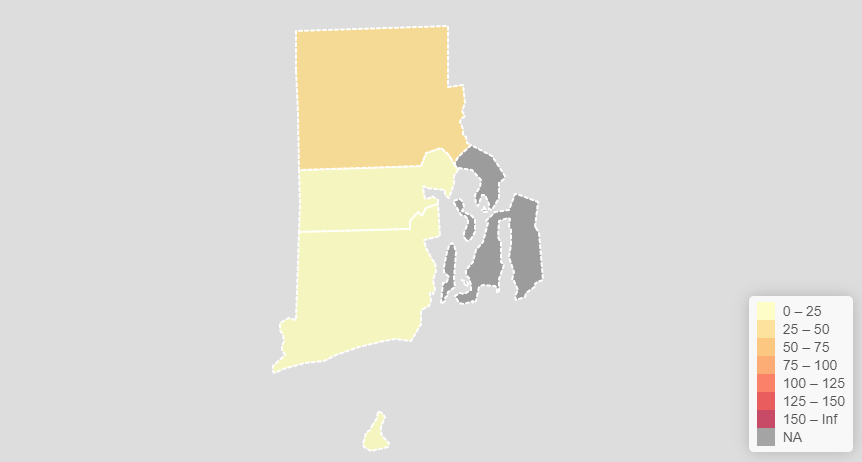
\includegraphics[width=.95\textwidth]{ImageResults/RhodeIsland100k.PNG}
    \captionof{figure}{Rhode Island: Number of Orphans per 100k Minors}
\end{minipage}
\subsubsection*{South Carolina}
\vfill
\hspace*{-3cm}
\begin{minipage}{.8\textwidth}
    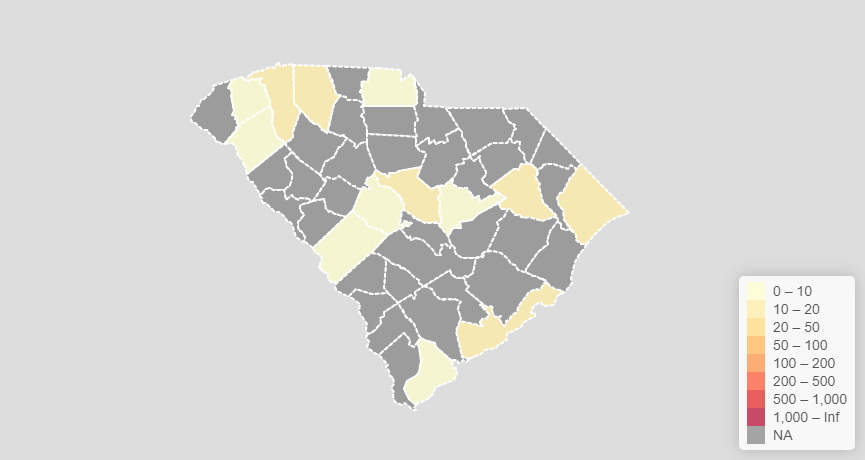
\includegraphics[width=.95\textwidth]{ImageResults/SouthCarolinaTotal.PNG}
    \captionof{figure}{South Carolina: Heat-map of Total Number of Orphans}
\end{minipage}%
\begin{minipage}{.8\textwidth}
    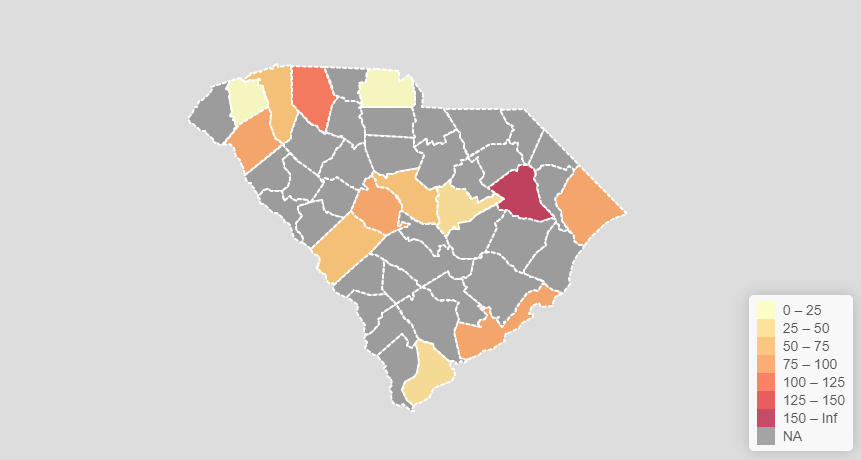
\includegraphics[width=.95\textwidth]{ImageResults/SouthCarolina100k.PNG}
    \captionof{figure}{South Carolina: Number of Orphans per 100k Minors}
\end{minipage}
\fillandplacepagenumber
\end{figure}
\end{landscape}

\begin{landscape}
\thispagestyle{empty}
\begin{figure}[h]
\subsubsection*{Tennessee}
\hspace*{-3cm}
\begin{minipage}{.8\textwidth}
    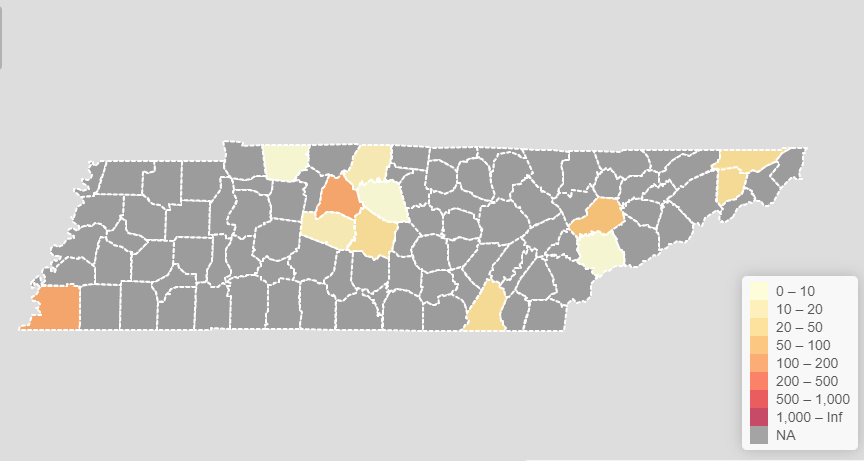
\includegraphics[width=.95\textwidth]{ImageResults/TennesseeTotal.PNG}
    \captionof{figure}{Tennessee: Heat-map of Total Number of Orphans}
\end{minipage}%
\begin{minipage}{.8\textwidth}
    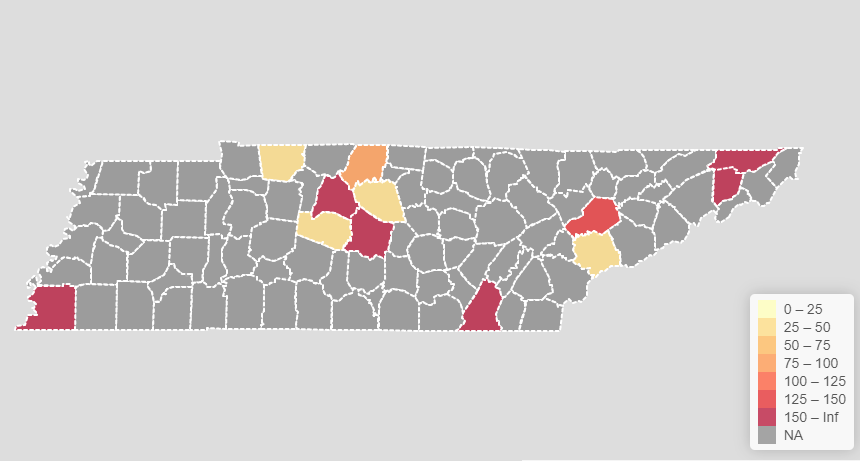
\includegraphics[width=.95\textwidth]{ImageResults/Tennessee100k.PNG}
    \captionof{figure}{Tennessee: Number of Orphans per 100k Minors}
\end{minipage}
\subsubsection*{Utah}
\vfill
\hspace*{-3cm}
\begin{minipage}{.8\textwidth}
    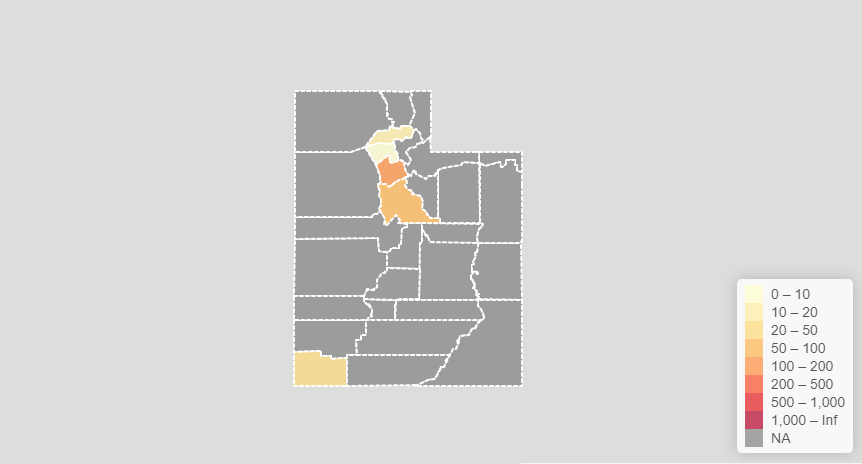
\includegraphics[width=.95\textwidth]{ImageResults/UtahTotal.PNG}
    \captionof{figure}{Utah: Heat-map of Total Number of Orphans}
\end{minipage}%
\begin{minipage}{.8\textwidth}
    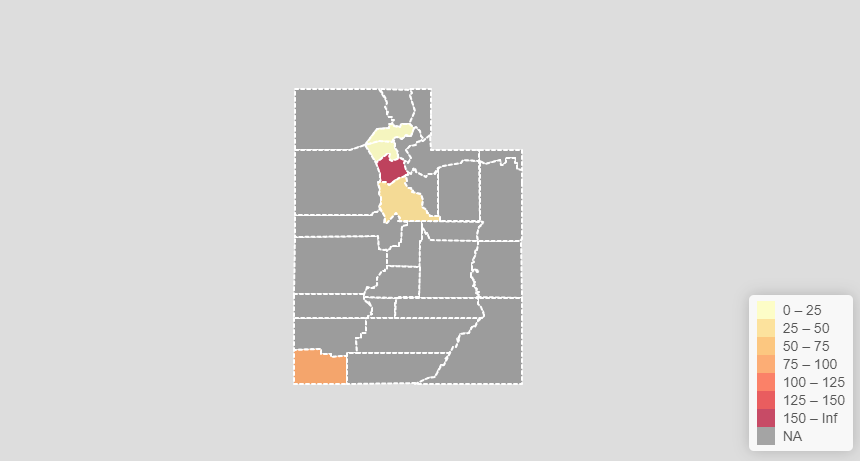
\includegraphics[width=.95\textwidth]{ImageResults/Utah100k.PNG}
    \captionof{figure}{Utah: Number of Orphans per 100k Minors}
\end{minipage}
\fillandplacepagenumber
\end{figure}
\end{landscape}



\newpage
\begin{figure}[H]
\subsubsection*{Washington}
\vspace{20pt}
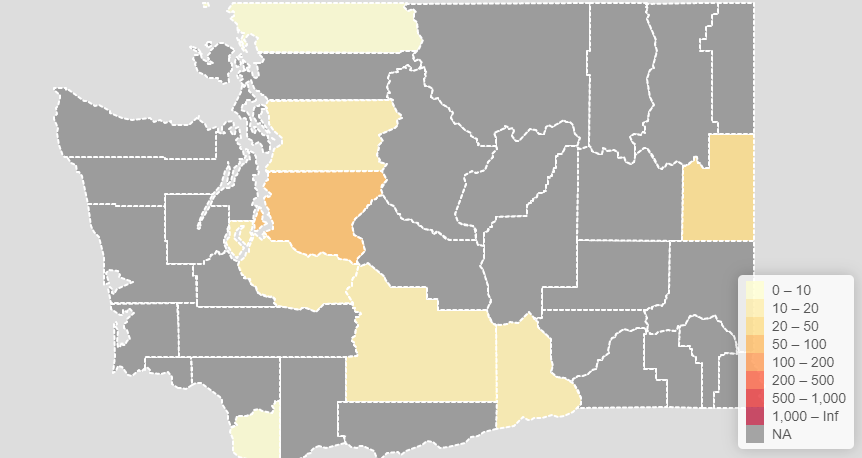
\includegraphics[width=0.95\textwidth]{ImageResults/WashingtonTotal.PNG}
\captionof{figure}{Washington: Heat-map of Total Number of Orphans}
\vspace{40pt}
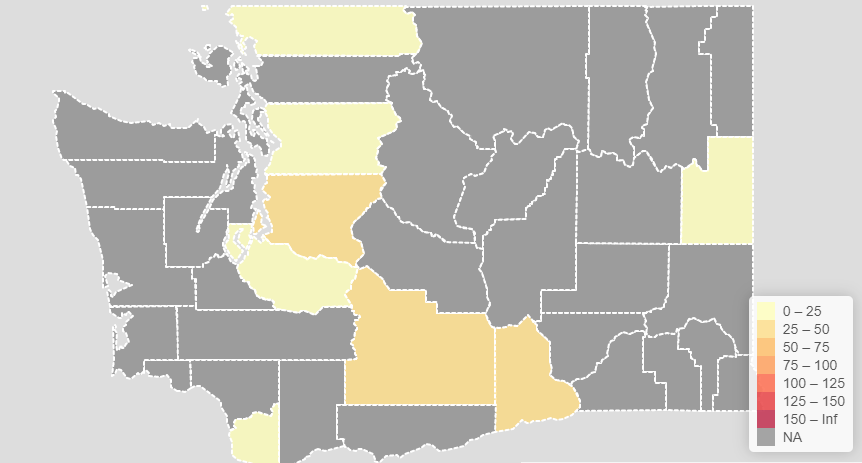
\includegraphics[width=0.95\textwidth]{ImageResults/Washington100k.PNG}
\captionof{figure}{Washington:  Number of Orphans per 100k Minors}
\end{figure}

%\newpage
\subsection{Discussion of Results}
\subsubsection{Limited Results}\label{s:limited results}
Providing a brief explanation as to why some data is missing (discussed further in later sections):

We collected natality and population data for 39 states but due to code limitations and lack of availability of computer memory we were unable to produce computed results for 22 of the states we collected data for. This could be fixed with access to a more powerful computed, or by changing the way the code runs, i.e. by improving efficiency of the code. This meant that we only have results for 17 states.

Many of the counties within states we managed to run have no result available and are displayed in grey. This is due to the lack of availability of the data: natality data is not available for counties with fewer than 100,000 residents. This means we are missing a huge chunk of the data and cannot get any results on low population counties. This can only be amended once the data does become available or if we extrapolate from counties with higher population.

\subsubsection{Implications of Results}
Although this project is does not perform any practical ‘plan of action’, these results provide import information from a practical viewpoint: it may allow one to construct a more appropriate plan to help combat the issues that surround COVID-19 induced orphanhood. The hotspots on the different counties show the worst impacted counties, thus informing which counties would require the most support to help the possible issues that the orphans may face. The results give clear insight into where is affected and it is clear to see from the results which areas have hotspots and which counties themselves have many hotspots.

From the maps (per 100k) we see generally the most affected areas are counties in or near major cities: for example, look at Massachusetts (see Figure~\ref{fig:Mass100k}), we have one ‘red’ area (Suffolk), which happens to be the centre of Boston. Also considering Maryland (see Figure~\ref{fig:Mary100k}), we see two red spots: one near the city Baltimore, and one in Montgomery, which contains some of the surrounding suburban area of Washington D.C.. This correlation is only a hypothesis and would need to be confirmed as a possible later experiment, however the aforementioned counties which have high orphanhood rates could be used straight away to help with a plan of action. 

Other than trends within counties, there is some larger scale possible correlation; some states have much higher overall orphanhood rates, namely Arizona, California and New Jersey (see Figures~\ref{fig:Ariz100k}, \ref{fig:Cali100k} and \ref{fig:Newj100k}). In these states there are many ‘red’ counties, and most counties generally have a much higher rate of orphanhood compared to other counties. It would be worth investigating if this has some correlation with population density or just a relation to the number of related COVID-19 deaths the state itself has. Although this is a future project, it is clear to see that these states have the highest rates, and are affected most by the related issues.  

\section{Evaluation and Further Research}

\subsection{Limitations of the Results}
There are limitations in how much we can interpret or trust the results. As mentioned in \ref{s:limited results}, results are not available for several counties, so the data we do see for each state may not be representative of that state. Also, Male fertility data was not collected until 2016, so we only collected male fertility data from 2016-2019, while we collected the data for 2003-2019 for females. We used a Poisson linear model based on the female data in order to extrapolate the male data for pre-2016, under the assumption that the model fits, which may cause some uncertainty.

We did not account for socioeconomic status in the study, however people in poverty tend to have higher fertility \cite{poverty_fertility}, and also higher COVID-19 related morbidity, which is affected by other social factors too \cite{social_covid19}. Accounting for these factors could potentially alter the results. Also, since these things have not been accounted for, in many cases it is difficult to explain why certain counties/states are disproportionately affected by COVID-19 related orphan cases, e.g. in some counties in California or Tennessee.

\subsection{Technical Challenges in the Approach}

A major technical hurdle was presented by missing data. This is a challenge that comes up often in larger-scale data analysis. In our case, computation of fertility and population data would take an unusually long time and sometimes cause the program to hang or to crash. Eventually we discovered that this was caused by merging large files with many blank lines (in place of where data should be). We were able to significantly increase efficiency and reduce computation time down to a workable level by removing blank lines before carrying out computation. Finding ways to increase efficiency like this is extremely important when working with large amounts of data.

Large states with many counties, such as Tennessee which has 95, could not be downloaded from the database as there was a limit of 75,000 lines per file. This problem was resolved by splitting the fertility/population data into several smaller files, each representing the data for a single year. For extremely large states, such as Texas - which has 254 counties and generated 90.2 MB of data in total - the data had to be split both by year and by race. However, this in turn meant that many data pulls had to be performed manually: 882 in total. The only way to resolve this was to divide the task among all 5 group members.

\subsection{Robustness and Longevity of the Solution}
While the issue of missing data was resolved, there are still some concerns over the robustness of the code when it comes to dealing with large files in general. To improve this, we could add a warning when the file that is about to be computed is very large or has many lines, or estimate the amount of free memory required to carry out the computation. This would reduce the risk of program/computer crashes and overflow errors.

The solution will remain usable and relevant in the future as there is a simple process to update data as newer or better data emerges: using git, one can simply replace the old files locally, "add" them, "commit" the changes and "push" them to the remote repository. Everyone with access to the project will be alerted of the changes. The code will not need to be amended at all provided that the data is formatted in the same way: as a column-headed text file, which is quite ubiquitous.

\subsection{Ways to Expand the Study}
In an identical way to how we would update the data, we could also add data for states that were not included in the original study due to constraints on computing resources and time. Since the repository is stored remotely, we could even give remote access to volunteers with more computing power in order to expand the study. Furthermore, the code is versatile enough that we could repeat the study for different countries, or even continents (replacing states by countries). The maps to produce the figures would need to be changed, but the code that computes the orphans estimate would be unchanged.

Where sufficient data is unavailable, for example for several counties in the original study, one could use extrapolation techniques to expand the the study. Since there is a high correlation (Pearson $r^2 = 0.94$) \cite{global_study} between the Total Fertility Rate and the ratio of orphans to COVID-19 related deaths, one could fit a linear model between these two variables using least squares estimates to estimate the parameters. Then, since COVID-19 deaths by US state \cite{covid_US_states} or county \cite{covid_US_counties} are readily available, we can use the model to estimate the number of orphans provided we have an estimate for the Total Fertility Rate. Similarly, we could extrapolate to other countries for which sufficient COVID-19 death data is available.

\subsection{Orphans Based on Race and Hispanic Origin}
When we originally pulled the data, we included groupings by race and Hispanic origin. With some modification to the code, we could display orphans by race for each county or state. This makes it easy for us in future to investigate if some races are disproportionately affected by COVID-19 related orphan cases. Since we have the data, we could also investigate differences in fertility and COVID-19 related morbidity between races in order to understand potential discrepancies. 

\subsection{Improving the model}
If data for orphan cases due to a caregiver dying from COVID-19 does become available, we could compare this data to the estimates from our model and update parts of the model appropriately. If the data is very different, we may have the amend the approach entirely. If new data emerges for specific parts of the model, for example the proportion of skip generation households, those can be updated easily by amending parameters in the code. 

\printbibliography 
\end{document}
